\documentclass[border=2pt]{standalone}
\usepackage{tikz}
\usetikzlibrary{arrows.meta}

% Brand color definitions (RGB 0-1 scale)
\definecolor{Garnet}{rgb}{0.451, 0.0, 0.039}
\definecolor{Atlantic}{rgb}{0.275, 0.416, 0.624}
\definecolor{Congaree}{rgb}{0.122, 0.255, 0.302}
\definecolor{Horseshoe}{rgb}{0.396, 0.471, 0.043}
\definecolor{Rose}{rgb}{0.8, 0.18, 0.251}
\definecolor{Honeycomb}{rgb}{0.643, 0.569, 0.216}
\definecolor{Grass}{rgb}{0.0, 0.8, 0.0}
\definecolor{Black90}{rgb}{0.212, 0.212, 0.212}
\definecolor{Black70}{rgb}{0.361, 0.361, 0.361}
\definecolor{Black50}{rgb}{0.635, 0.635, 0.635}

\begin{document}

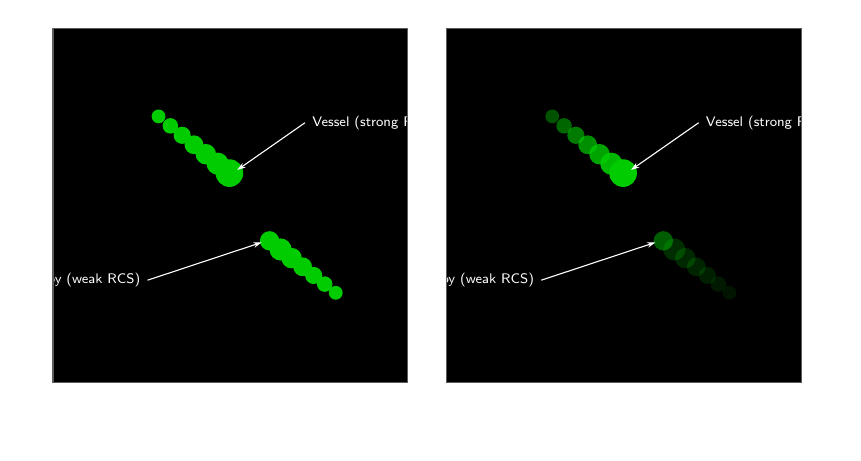
\begin{tikzpicture}[font=\sffamily\footnotesize]

  % -------------------------------------------------------
  % Panel (a): Binary encoding
  % -------------------------------------------------------
  \begin{scope}[xshift=0cm]

    % Black background panel
    \fill[black] (0,0) rectangle (4.5,4.5);

    % --- Strong target (vessel) at upper-left ~(1.2, 3.2) ---
    % Vessel current position: (2.24, 2.66)
    % Trail step reduced to ~55% of original: (-0.15, +0.12) per age step
    % age 6 (oldest) ... age 1 (newest trail)
    % Binary: all trail dots full Grass opacity, size increases toward current
    \fill[Grass, opacity=1.0] (1.34, 3.38) circle (2.5pt);   % age 6 (oldest)
    \fill[Grass, opacity=1.0] (1.49, 3.26) circle (2.8pt);   % age 5
    \fill[Grass, opacity=1.0] (1.64, 3.14) circle (3.1pt);   % age 4
    \fill[Grass, opacity=1.0] (1.79, 3.02) circle (3.4pt);   % age 3
    \fill[Grass, opacity=1.0] (1.94, 2.90) circle (3.7pt);   % age 2
    \fill[Grass, opacity=1.0] (2.09, 2.78) circle (4.0pt);   % age 1 (newest trail)
    % Current vessel target
    \fill[Grass] (2.24, 2.66) circle (5pt);

    % --- Weak target (buoy) at lower-right ~(3.2, 1.4) ---
    % Buoy current position: (2.75, 1.80)
    % Trail step reduced to ~55% of original: (+0.14, -0.11) per age step
    % Binary: all trail dots full Grass opacity
    \fill[Grass, opacity=1.0] (3.59, 1.14) circle (2.5pt);   % age 6 (oldest)
    \fill[Grass, opacity=1.0] (3.45, 1.25) circle (2.8pt);   % age 5
    \fill[Grass, opacity=1.0] (3.31, 1.36) circle (3.1pt);   % age 4
    \fill[Grass, opacity=1.0] (3.17, 1.47) circle (3.4pt);   % age 3
    \fill[Grass, opacity=1.0] (3.03, 1.58) circle (3.7pt);   % age 2
    \fill[Grass, opacity=1.0] (2.89, 1.69) circle (4.0pt);   % age 1
    % Current buoy target (smaller)
    \fill[Grass] (2.75, 1.80) circle (3.5pt);

    % Annotations with white arrows
    % Vessel annotation: label to the right, arrow pointing left to vessel
    \draw[white, -{Stealth[length=3pt,width=2pt]}, line width=0.4pt]
      (3.20, 3.30) -- (2.34, 2.70);
    \node[white, anchor=west, inner sep=1pt] at (3.25, 3.30)
      {\tiny Vessel (strong RCS)};

    % Buoy annotation: label to the left, arrow pointing right to buoy
    \draw[white, -{Stealth[length=3pt,width=2pt]}, line width=0.4pt]
      (1.20, 1.30) -- (2.65, 1.78);
    \node[white, anchor=east, inner sep=1pt] at (1.15, 1.30)
      {\tiny Buoy (weak RCS)};

    % Panel border
    \draw[Black70, line width=0.4pt] (0,0) rectangle (4.5,4.5);

    % Panel title below
    \node[white, anchor=north] at (2.25, -0.12)
      {\footnotesize (a) Binary encoding};

  \end{scope}

  % -------------------------------------------------------
  % Panel (b): Proportional encoding
  % -------------------------------------------------------
  \begin{scope}[xshift=5.0cm]

    % Black background panel
    \fill[black] (0,0) rectangle (4.5,4.5);

    % --- Strong target (vessel): bright trail, opacity decays with age ---
    % age opacity: newest=0.9, stepping down to oldest=0.4
    % Trail positions same as panel (a)
    \fill[Grass, opacity=0.40] (1.34, 3.38) circle (2.5pt);   % age 6 (oldest)
    \fill[Grass, opacity=0.50] (1.49, 3.26) circle (2.8pt);   % age 5
    \fill[Grass, opacity=0.60] (1.64, 3.14) circle (3.1pt);   % age 4
    \fill[Grass, opacity=0.70] (1.79, 3.02) circle (3.4pt);   % age 3
    \fill[Grass, opacity=0.80] (1.94, 2.90) circle (3.7pt);   % age 2
    \fill[Grass, opacity=0.90] (2.09, 2.78) circle (4.0pt);   % age 1
    % Current vessel target
    \fill[Grass] (2.24, 2.66) circle (5pt);

    % --- Weak target (buoy): dim trail, base opacity 0.25, further decays ---
    % age opacity: newest=0.25*0.9=0.225, oldest=0.25*0.4=0.10
    \fill[Grass, opacity=0.10]  (3.59, 1.14) circle (2.5pt);  % age 6 (oldest)
    \fill[Grass, opacity=0.125] (3.45, 1.25) circle (2.8pt);  % age 5
    \fill[Grass, opacity=0.15]  (3.31, 1.36) circle (3.1pt);  % age 4
    \fill[Grass, opacity=0.175] (3.17, 1.47) circle (3.4pt);  % age 3
    \fill[Grass, opacity=0.20]  (3.03, 1.58) circle (3.7pt);  % age 2
    \fill[Grass, opacity=0.225] (2.89, 1.69) circle (4.0pt);  % age 1
    % Current buoy target (smaller, dim)
    \fill[Grass, opacity=0.45] (2.75, 1.80) circle (3.5pt);

    % Annotations
    \draw[white, -{Stealth[length=3pt,width=2pt]}, line width=0.4pt]
      (3.20, 3.30) -- (2.34, 2.70);
    \node[white, anchor=west, inner sep=1pt] at (3.25, 3.30)
      {\tiny Vessel (strong RCS)};

    \draw[white, -{Stealth[length=3pt,width=2pt]}, line width=0.4pt]
      (1.20, 1.30) -- (2.65, 1.78);
    \node[white, anchor=east, inner sep=1pt] at (1.15, 1.30)
      {\tiny Buoy (weak RCS)};

    % Panel border
    \draw[Black70, line width=0.4pt] (0,0) rectangle (4.5,4.5);

    % Panel title below
    \node[white, anchor=north] at (2.25, -0.12)
      {\footnotesize (b) Proportional encoding};

  \end{scope}

\end{tikzpicture}

\end{document}
